\chapter{Node.js and MongoDB CRUD  application}
%Intro\footnotemark\\
\par Lorem ipsum dolor sit amet, consectetur adipiscing elit. Aliquam facilisis massa quis orci volutpat, ut dictum tellus pulvinar. Nam vulputate diam a leo dignissim varius. Aenean nec tellus malesuada, tristique libero vitae, lacinia nibh. Donec quam libero, accumsan sollicitudin massa a, dictum gravida mauris.
\begin{spacing}{1.2}
%note en bas de page
\section{Implementing Endpoints }
\par Lorem ipsum dolor sit amet, consectetur adipiscing elit. Aliquam facilisis massa quis orci volutpat, ut dictum tellus pulvinar. Nam vulputate diam a leo dignissim varius. Aenean nec tellus malesuada, tristique libero vitae, lacinia nibh. Donec quam libero, accumsan sollicitudin massa a, dictum gravida mauris
\\
\begin{figure}[!htb] 
\begin{center} 
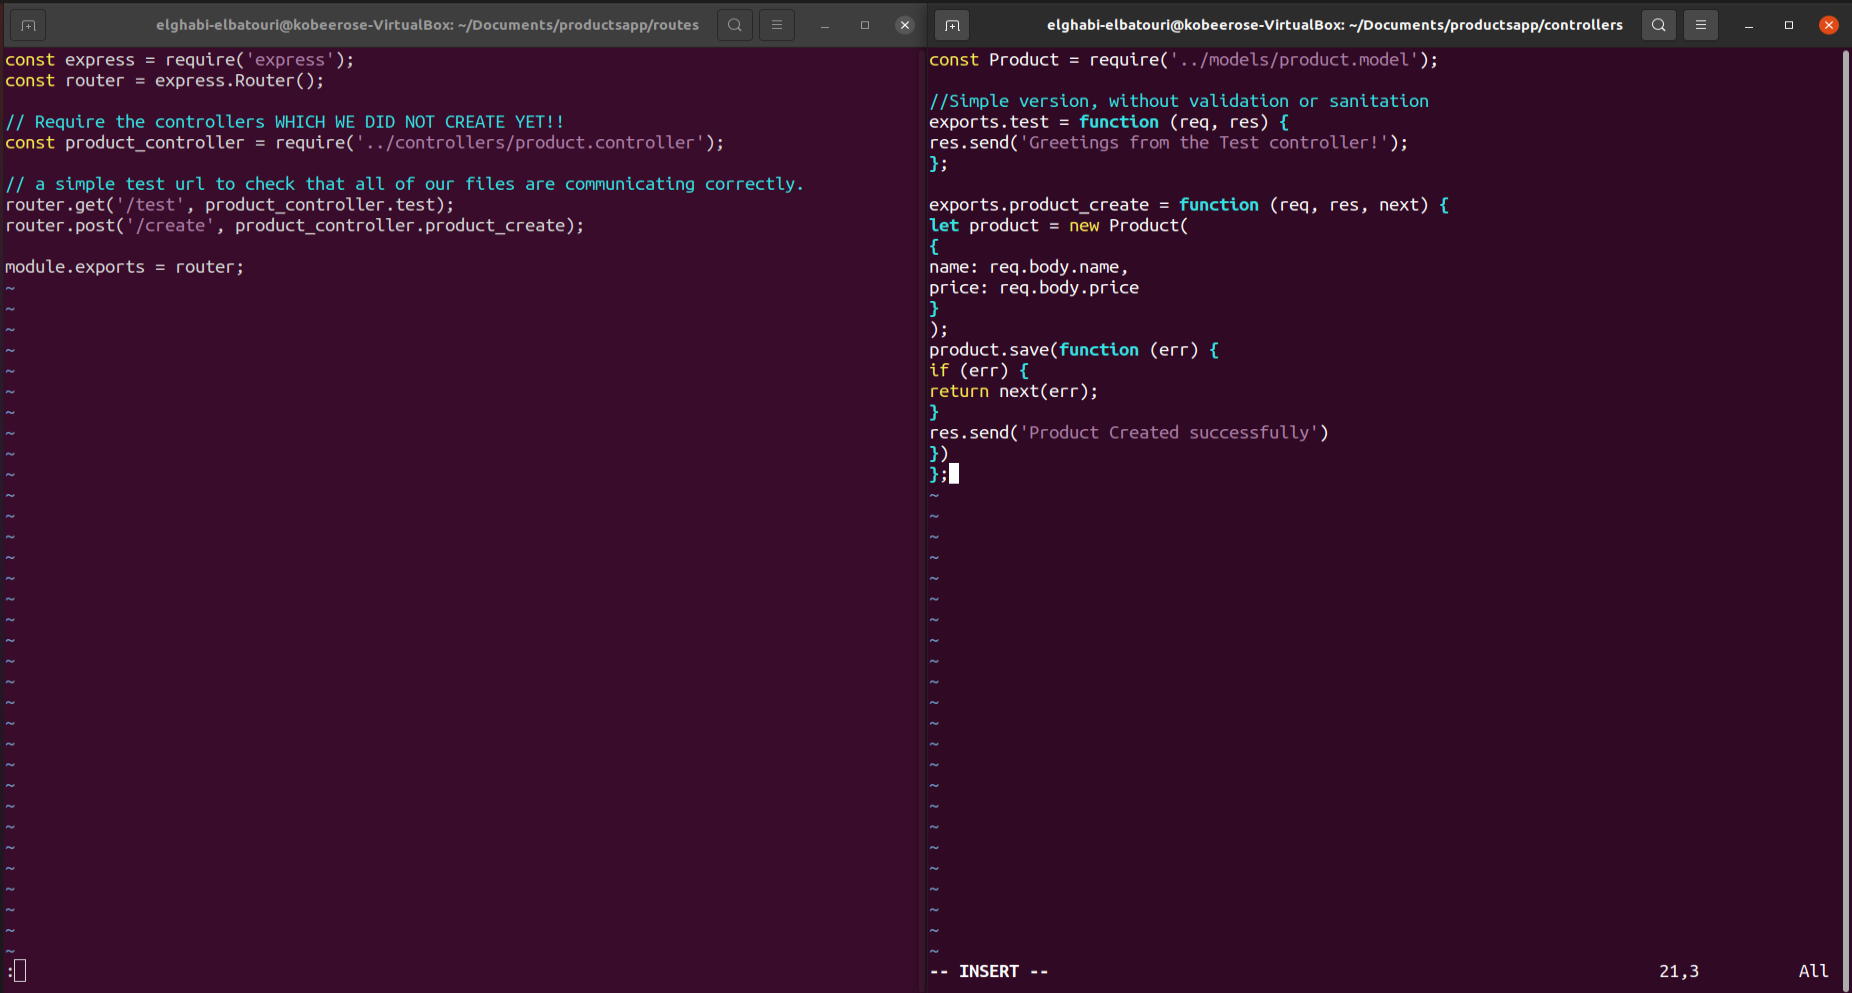
\includegraphics[width=1\linewidth]{Pictures/MongoDB/Node.js and MongoDB CRUD  application/Implementing Endpoints/Router and Controller for CREATE} 
\end{center} 
\caption{Router and Controller for CREATE} 
\end{figure}  \FloatBarrier
\\

\par Lorem ipsum dolor sit amet, consectetur adipiscing elit. Aliquam facilisis massa quis orci volutpat, ut dictum tellus pulvinar. Nam vulputate diam a leo dignissim varius. Aenean nec tellus malesuada, tristique libero vitae, lacinia nibh. Donec quam libero, accumsan sollicitudin massa a, dictum gravida mauris
\\
\begin{figure}[!htb] 
\begin{center} 
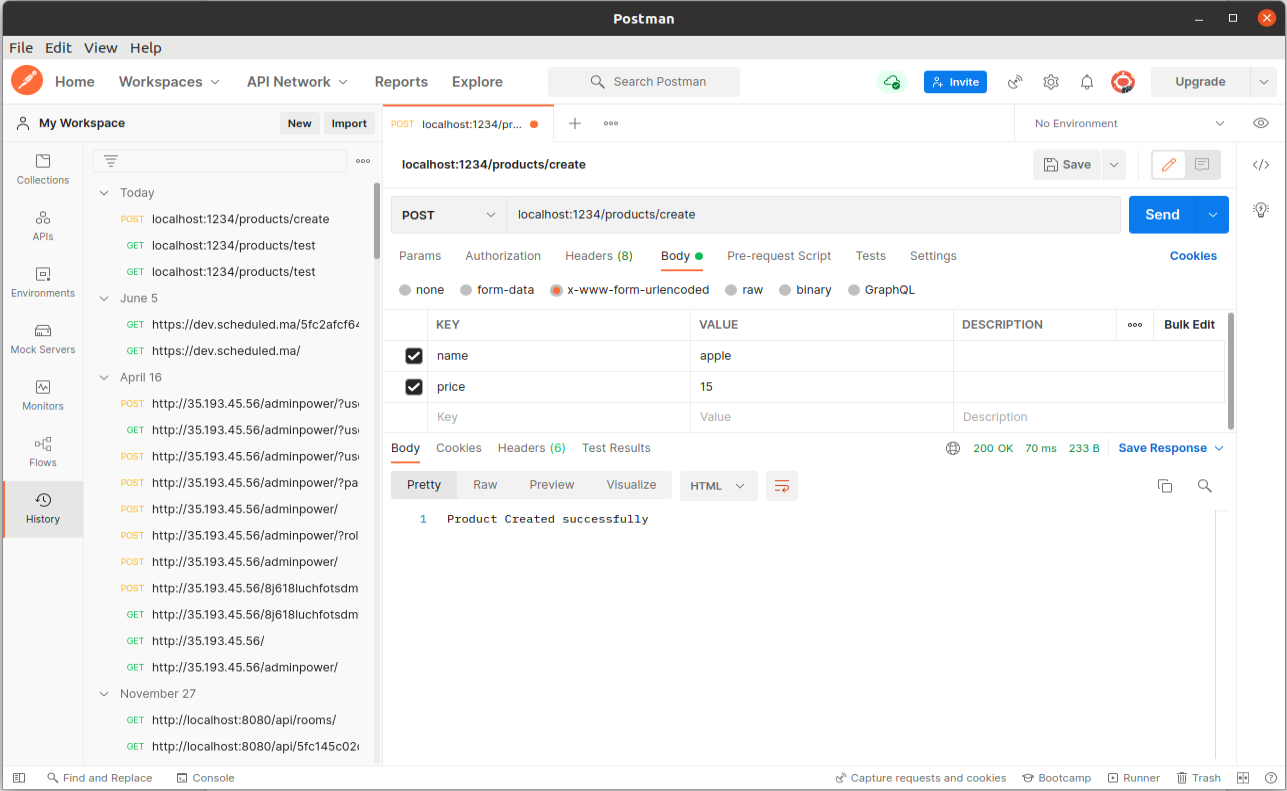
\includegraphics[width=1\linewidth]{Pictures/MongoDB/Node.js and MongoDB CRUD  application/Implementing Endpoints/Testing CREATE endpoint} 
\end{center} 
\caption{Testing CREATE endpoint} 
\end{figure}  \FloatBarrier
\\

\par Lorem ipsum dolor sit amet, consectetur adipiscing elit. Aliquam facilisis massa quis orci volutpat, ut dictum tellus pulvinar. Nam vulputate diam a leo dignissim varius. Aenean nec tellus malesuada, tristique libero vitae, lacinia nibh. Donec quam libero, accumsan sollicitudin massa a, dictum gravida mauris
\\
\begin{figure}[!htb] 
\begin{center} 
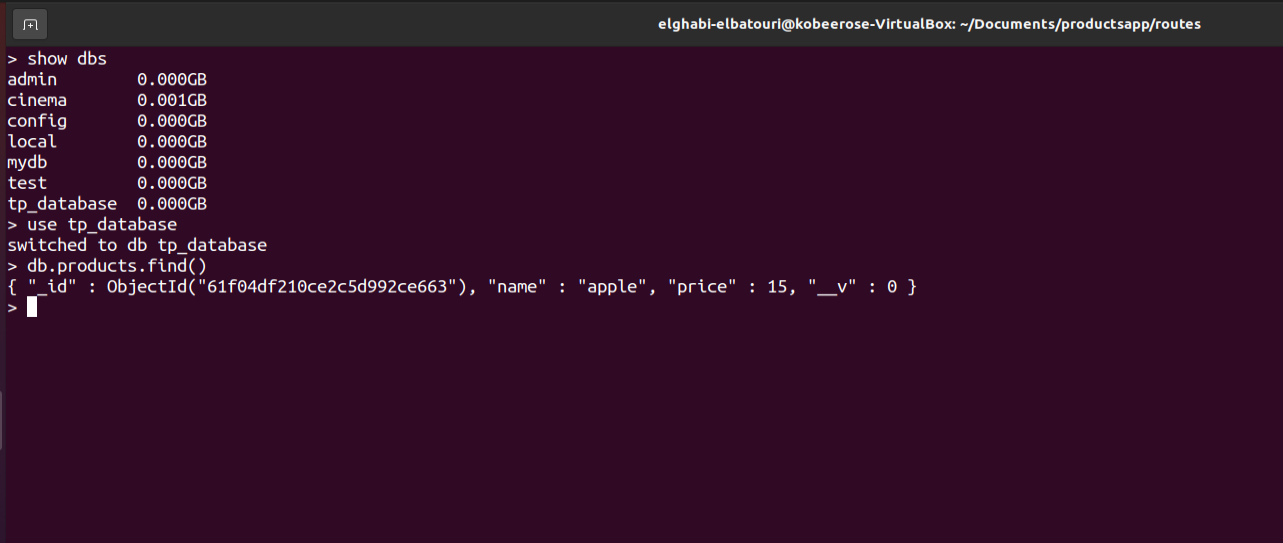
\includegraphics[width=1\linewidth]{Pictures/MongoDB/Node.js and MongoDB CRUD  application/Implementing Endpoints/Finding new object in MongoDB} 
\end{center} 
\caption{Finding new object in MongoDB} 
\end{figure}  \FloatBarrier
\\

\par Lorem ipsum dolor sit amet, consectetur adipiscing elit. Aliquam facilisis massa quis orci volutpat, ut dictum tellus pulvinar. Nam vulputate diam a leo dignissim varius. Aenean nec tellus malesuada, tristique libero vitae, lacinia nibh. Donec quam libero, accumsan sollicitudin massa a, dictum gravida mauris
\\
\begin{figure}[!htb] 
\begin{center} 
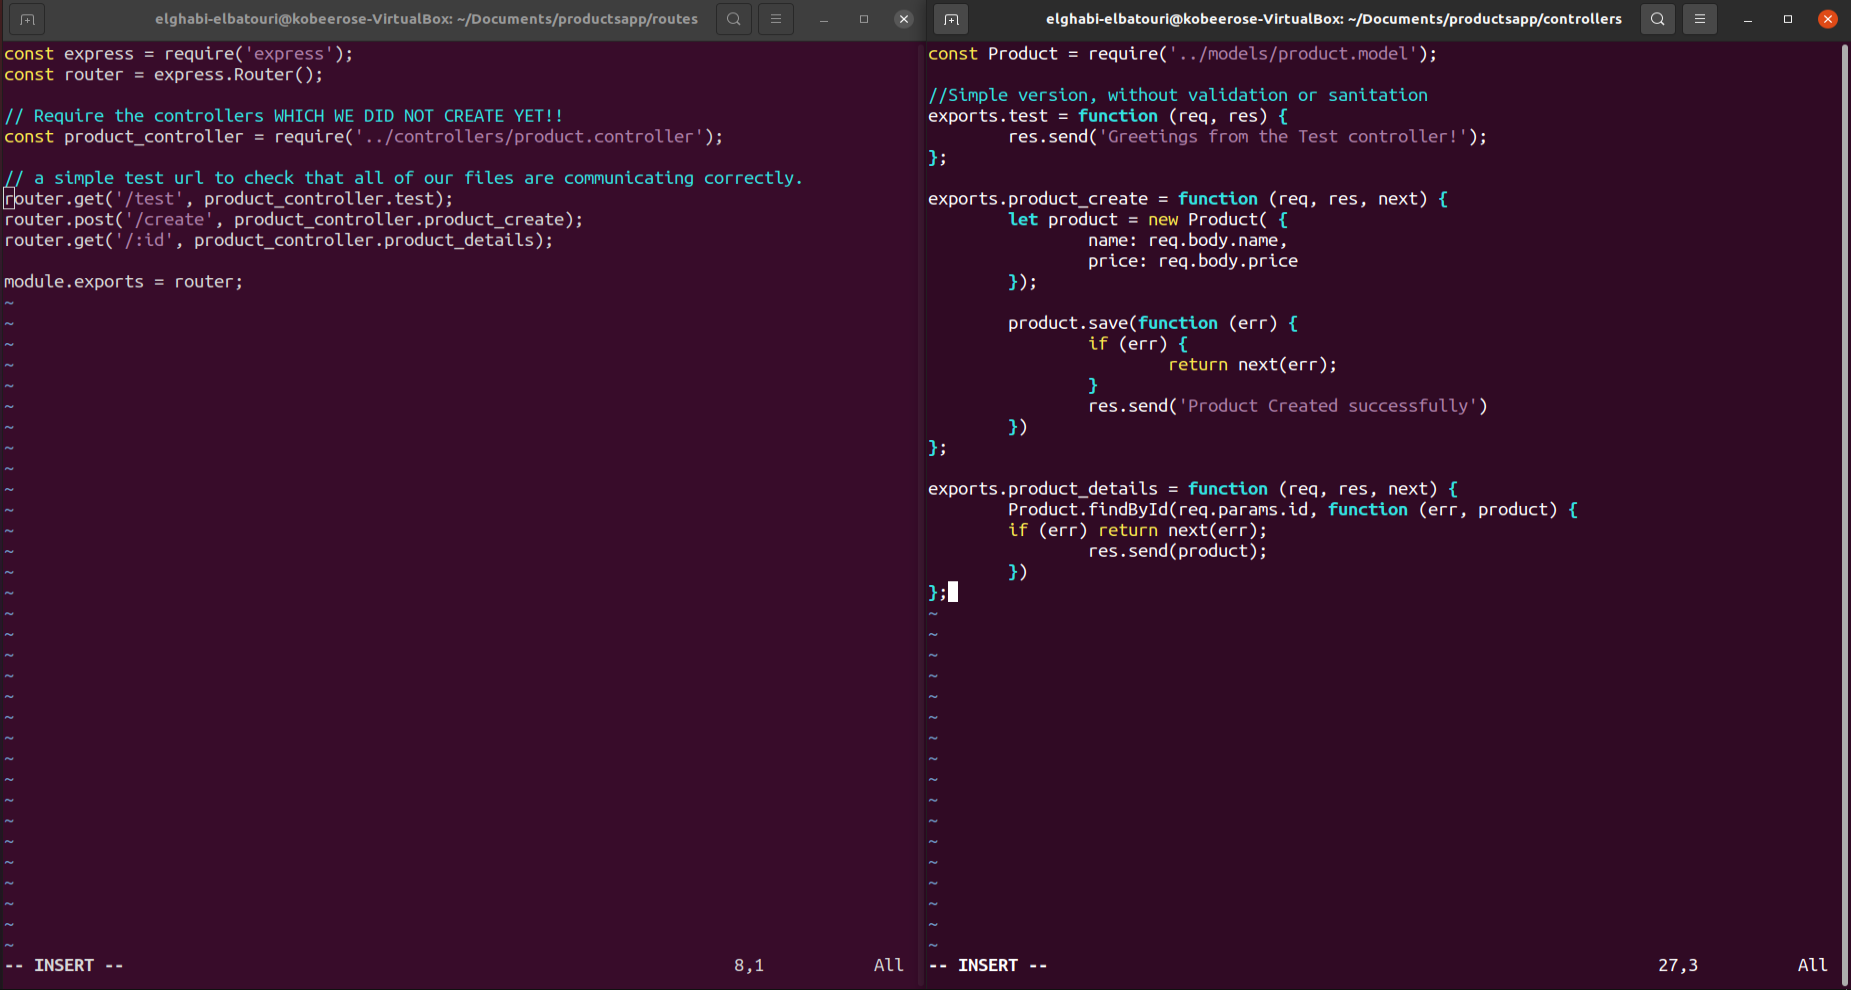
\includegraphics[width=1\linewidth]{Pictures/MongoDB/Node.js and MongoDB CRUD  application/Implementing Endpoints/Router and Controller for READ} 
\end{center} 
\caption{Router and Controller for READ} 
\end{figure}  \FloatBarrier
\\

\par Lorem ipsum dolor sit amet, consectetur adipiscing elit. Aliquam facilisis massa quis orci volutpat, ut dictum tellus pulvinar. Nam vulputate diam a leo dignissim varius. Aenean nec tellus malesuada, tristique libero vitae, lacinia nibh. Donec quam libero, accumsan sollicitudin massa a, dictum gravida mauris
\\
\begin{figure}[!htb] 
\begin{center} 
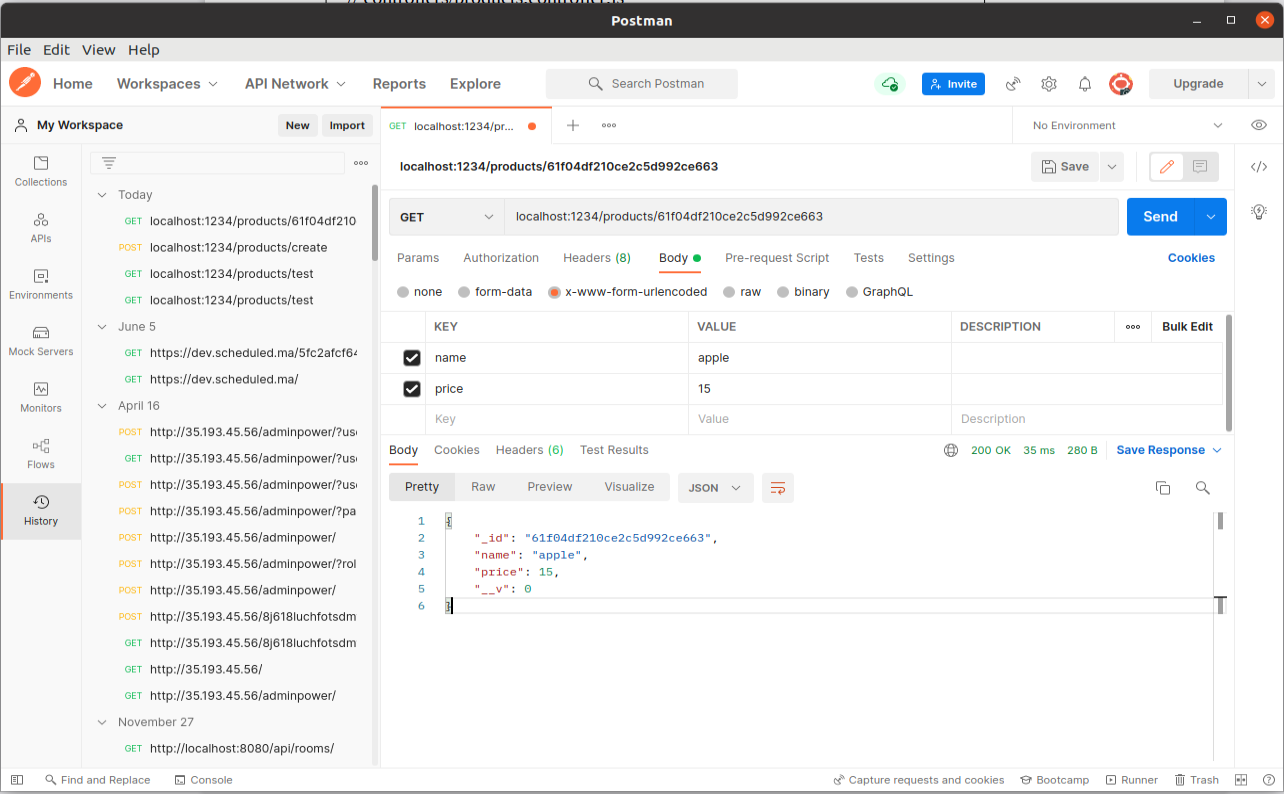
\includegraphics[width=1\linewidth]{Pictures/MongoDB/Node.js and MongoDB CRUD  application/Implementing Endpoints/Testing READ endpoint} 
\end{center} 
\caption{Testing READ endpoint} 
\end{figure}  \FloatBarrier
\\

\par Lorem ipsum dolor sit amet, consectetur adipiscing elit. Aliquam facilisis massa quis orci volutpat, ut dictum tellus pulvinar. Nam vulputate diam a leo dignissim varius. Aenean nec tellus malesuada, tristique libero vitae, lacinia nibh. Donec quam libero, accumsan sollicitudin massa a, dictum gravida mauris
\\
\begin{figure}[!htb] 
\begin{center} 
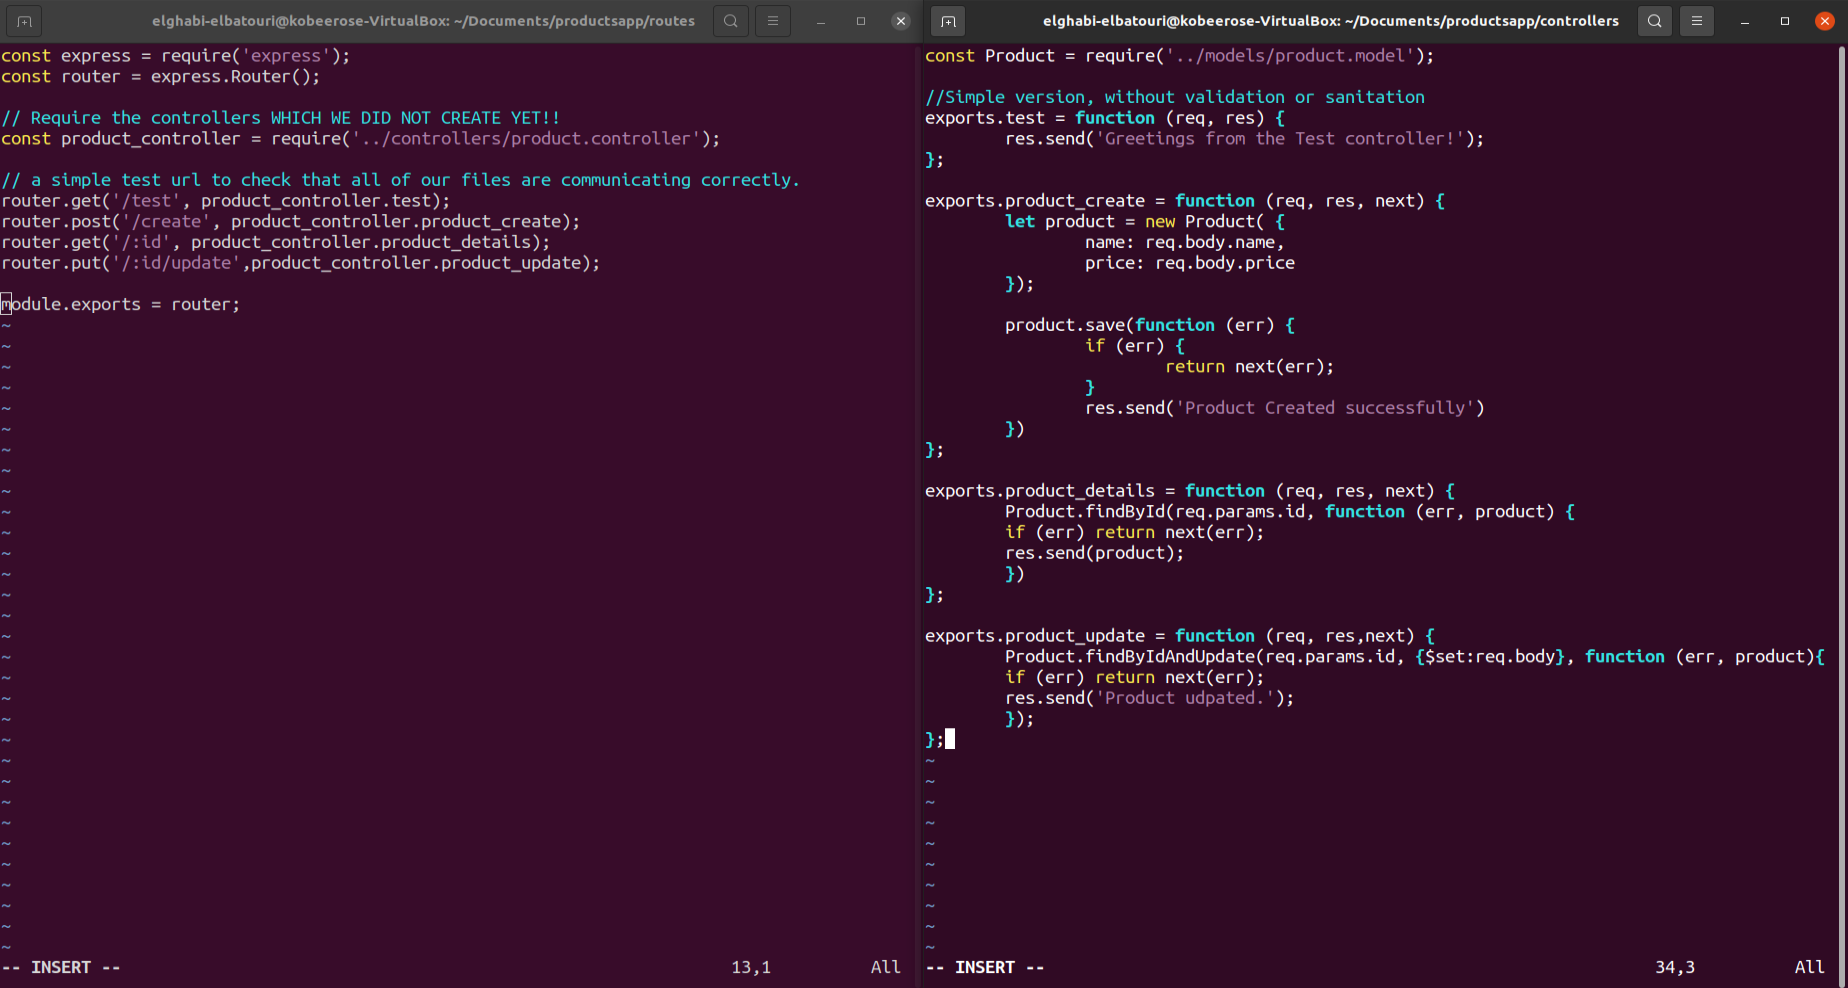
\includegraphics[width=1\linewidth]{Pictures/MongoDB/Node.js and MongoDB CRUD  application/Implementing Endpoints/Router and Controller for UPDATE} 
\end{center} 
\caption{Router and Controller for UPDATE} 
\end{figure}  \FloatBarrier
\\

\par Lorem ipsum dolor sit amet, consectetur adipiscing elit. Aliquam facilisis massa quis orci volutpat, ut dictum tellus pulvinar. Nam vulputate diam a leo dignissim varius. Aenean nec tellus malesuada, tristique libero vitae, lacinia nibh. Donec quam libero, accumsan sollicitudin massa a, dictum gravida mauris
\\
\begin{figure}[!htb] 
\begin{center} 
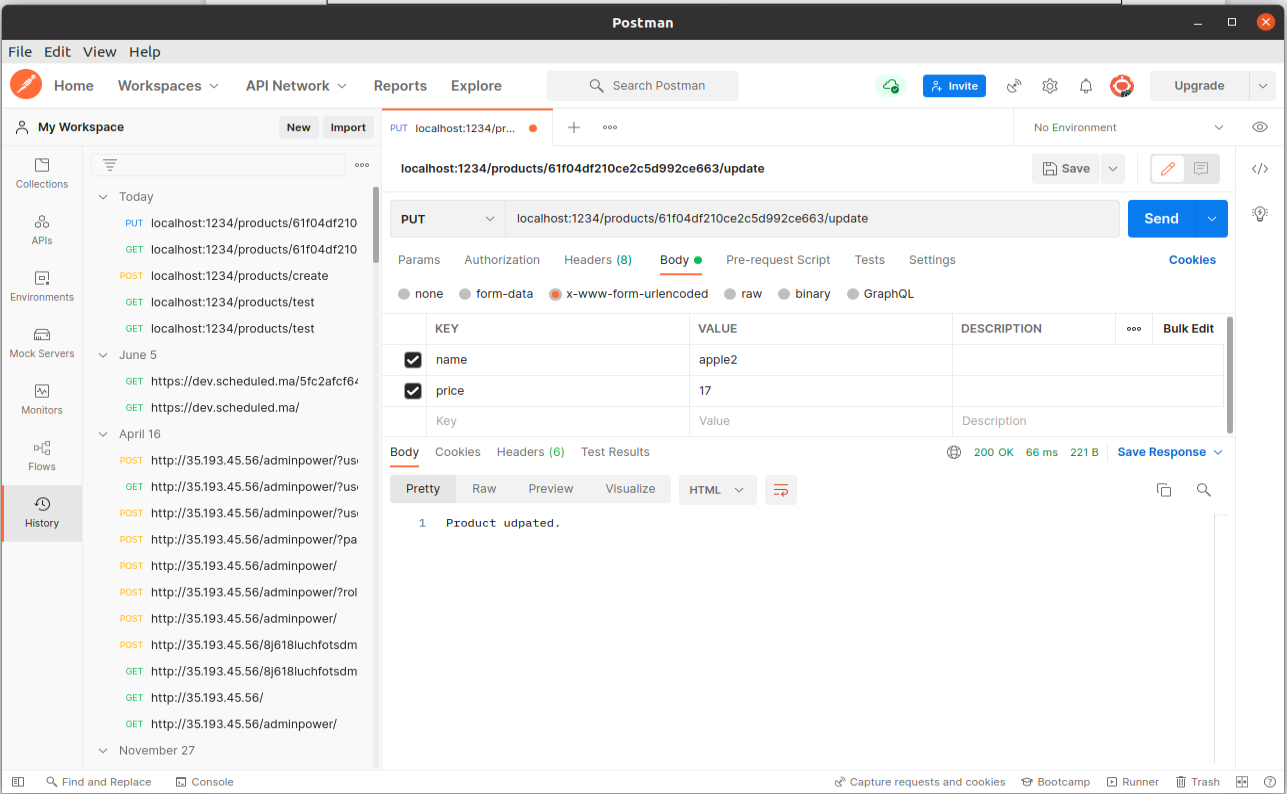
\includegraphics[width=1\linewidth]{Pictures/MongoDB/Node.js and MongoDB CRUD  application/Implementing Endpoints/Testing UPDATE endpoint} 
\end{center} 
\caption{Testing UPDATE endpoint} 
\end{figure}  \FloatBarrier
\\

\par Lorem ipsum dolor sit amet, consectetur adipiscing elit. Aliquam facilisis massa quis orci volutpat, ut dictum tellus pulvinar. Nam vulputate diam a leo dignissim varius. Aenean nec tellus malesuada, tristique libero vitae, lacinia nibh. Donec quam libero, accumsan sollicitudin massa a, dictum gravida mauris
\\
\begin{figure}[!htb] 
\begin{center} 
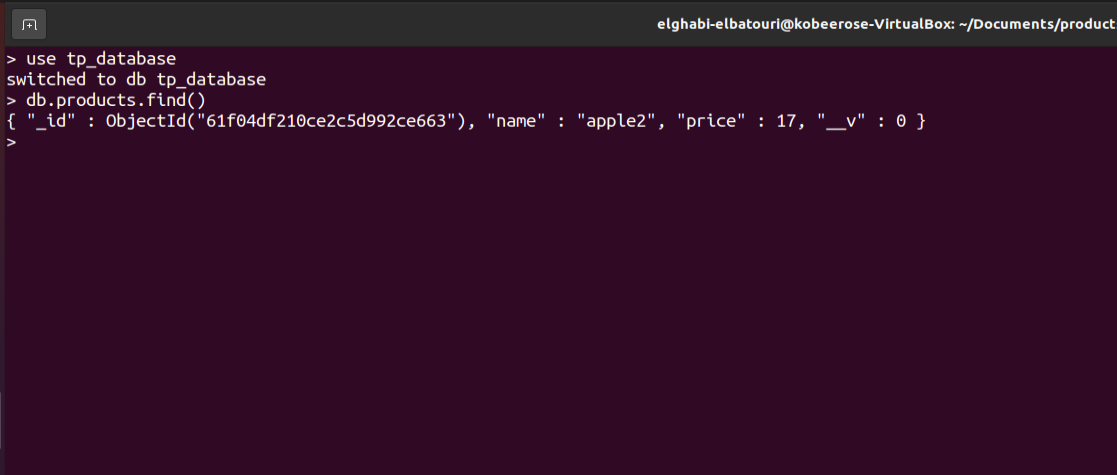
\includegraphics[width=1\linewidth]{Pictures/MongoDB/Node.js and MongoDB CRUD  application/Implementing Endpoints/Verifying Changes in MongoDB} 
\end{center} 
\caption{Verifying Changes in MongoDB} 
\end{figure}  \FloatBarrier
\\

\par Lorem ipsum dolor sit amet, consectetur adipiscing elit. Aliquam facilisis massa quis orci volutpat, ut dictum tellus pulvinar. Nam vulputate diam a leo dignissim varius. Aenean nec tellus malesuada, tristique libero vitae, lacinia nibh. Donec quam libero, accumsan sollicitudin massa a, dictum gravida mauris
\\
\begin{figure}[!htb] 
\begin{center} 
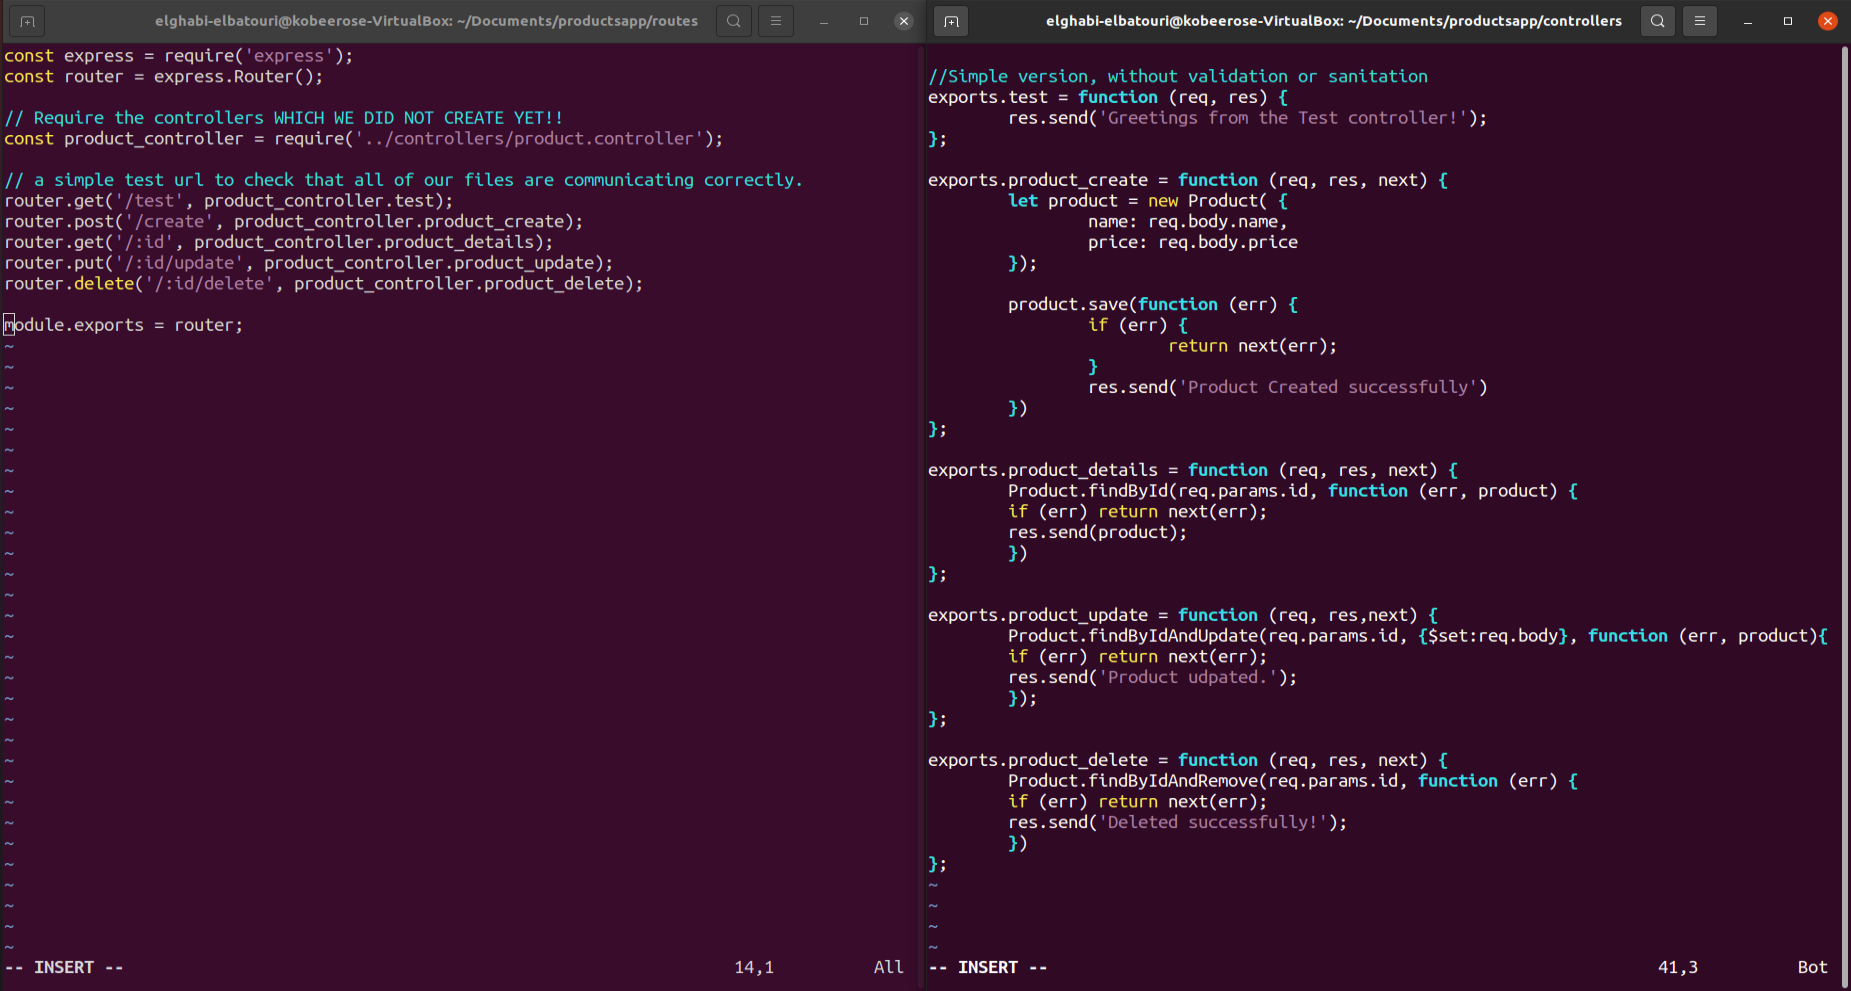
\includegraphics[width=1\linewidth]{Pictures/MongoDB/Node.js and MongoDB CRUD  application/Implementing Endpoints/Router and Controller for DELETE} 
\end{center} 
\caption{Router and Controller for DELETE} 
\end{figure}  \FloatBarrier
\\

\par Lorem ipsum dolor sit amet, consectetur adipiscing elit. Aliquam facilisis massa quis orci volutpat, ut dictum tellus pulvinar. Nam vulputate diam a leo dignissim varius. Aenean nec tellus malesuada, tristique libero vitae, lacinia nibh. Donec quam libero, accumsan sollicitudin massa a, dictum gravida mauris
\\
\begin{figure}[!htb] 
\begin{center} 
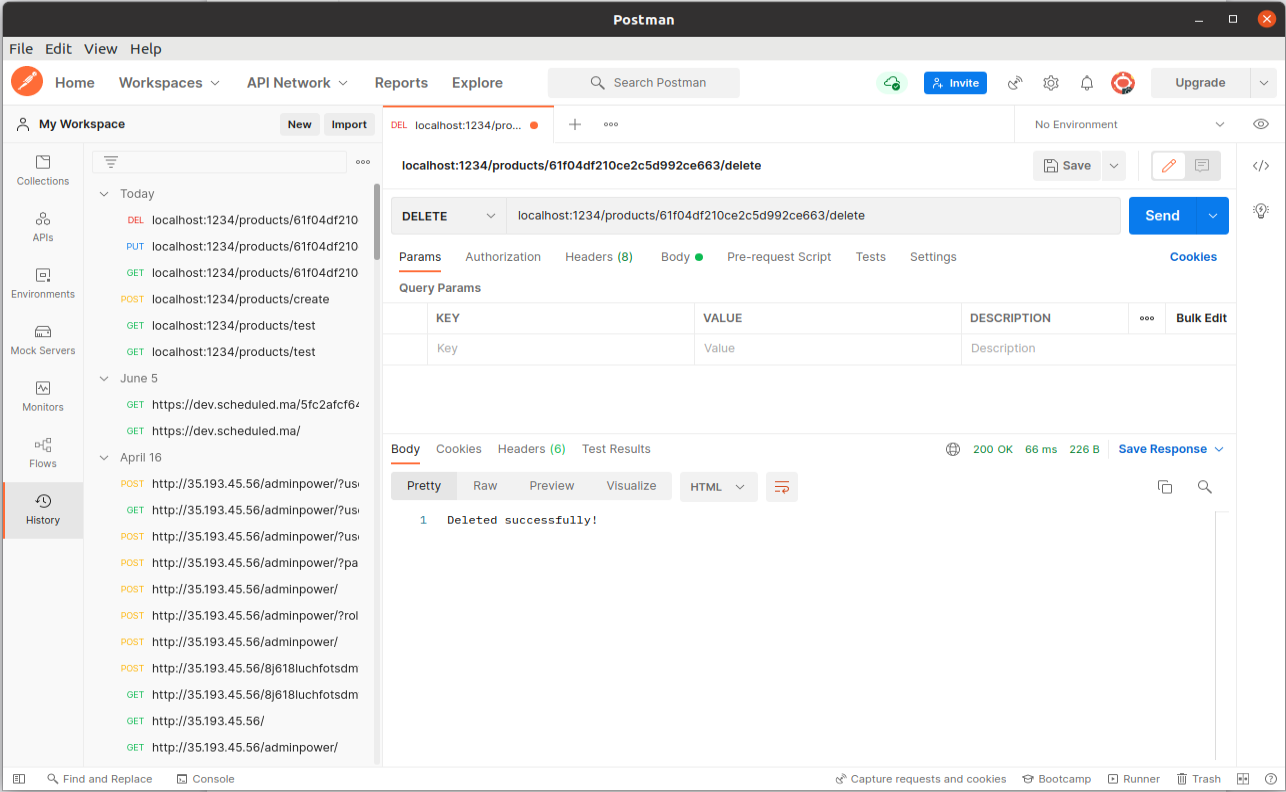
\includegraphics[width=1\linewidth]{Pictures/MongoDB/Node.js and MongoDB CRUD  application/Implementing Endpoints/Testing DELETE endpoint} 
\end{center} 
\caption{Testing DELETE endpoint} 
\end{figure}  \FloatBarrier
\\

\par Lorem ipsum dolor sit amet, consectetur adipiscing elit. Aliquam facilisis massa quis orci volutpat, ut dictum tellus pulvinar. Nam vulputate diam a leo dignissim varius. Aenean nec tellus malesuada, tristique libero vitae, lacinia nibh. Donec quam libero, accumsan sollicitudin massa a, dictum gravida mauris
\\
\begin{figure}[!htb] 
\begin{center} 
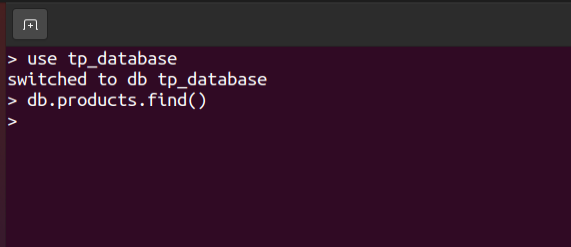
\includegraphics[width=1\linewidth]{Pictures/MongoDB/Node.js and MongoDB CRUD  application/Implementing Endpoints/Empty db in mongo} 
\end{center} 
\caption{Empty db in mongo} 
\end{figure}  \FloatBarrier
\\
\section{Node.js installation }
\par Lorem ipsum dolor sit amet, consectetur adipiscing elit. Aliquam facilisis massa quis orci volutpat, ut dictum tellus pulvinar. Nam vulputate diam a leo dignissim varius. Aenean nec tellus malesuada, tristique libero vitae, lacinia nibh. Donec quam libero, accumsan sollicitudin massa a, dictum gravida mauris
\\
\begin{figure}[!htb] 
\begin{center} 
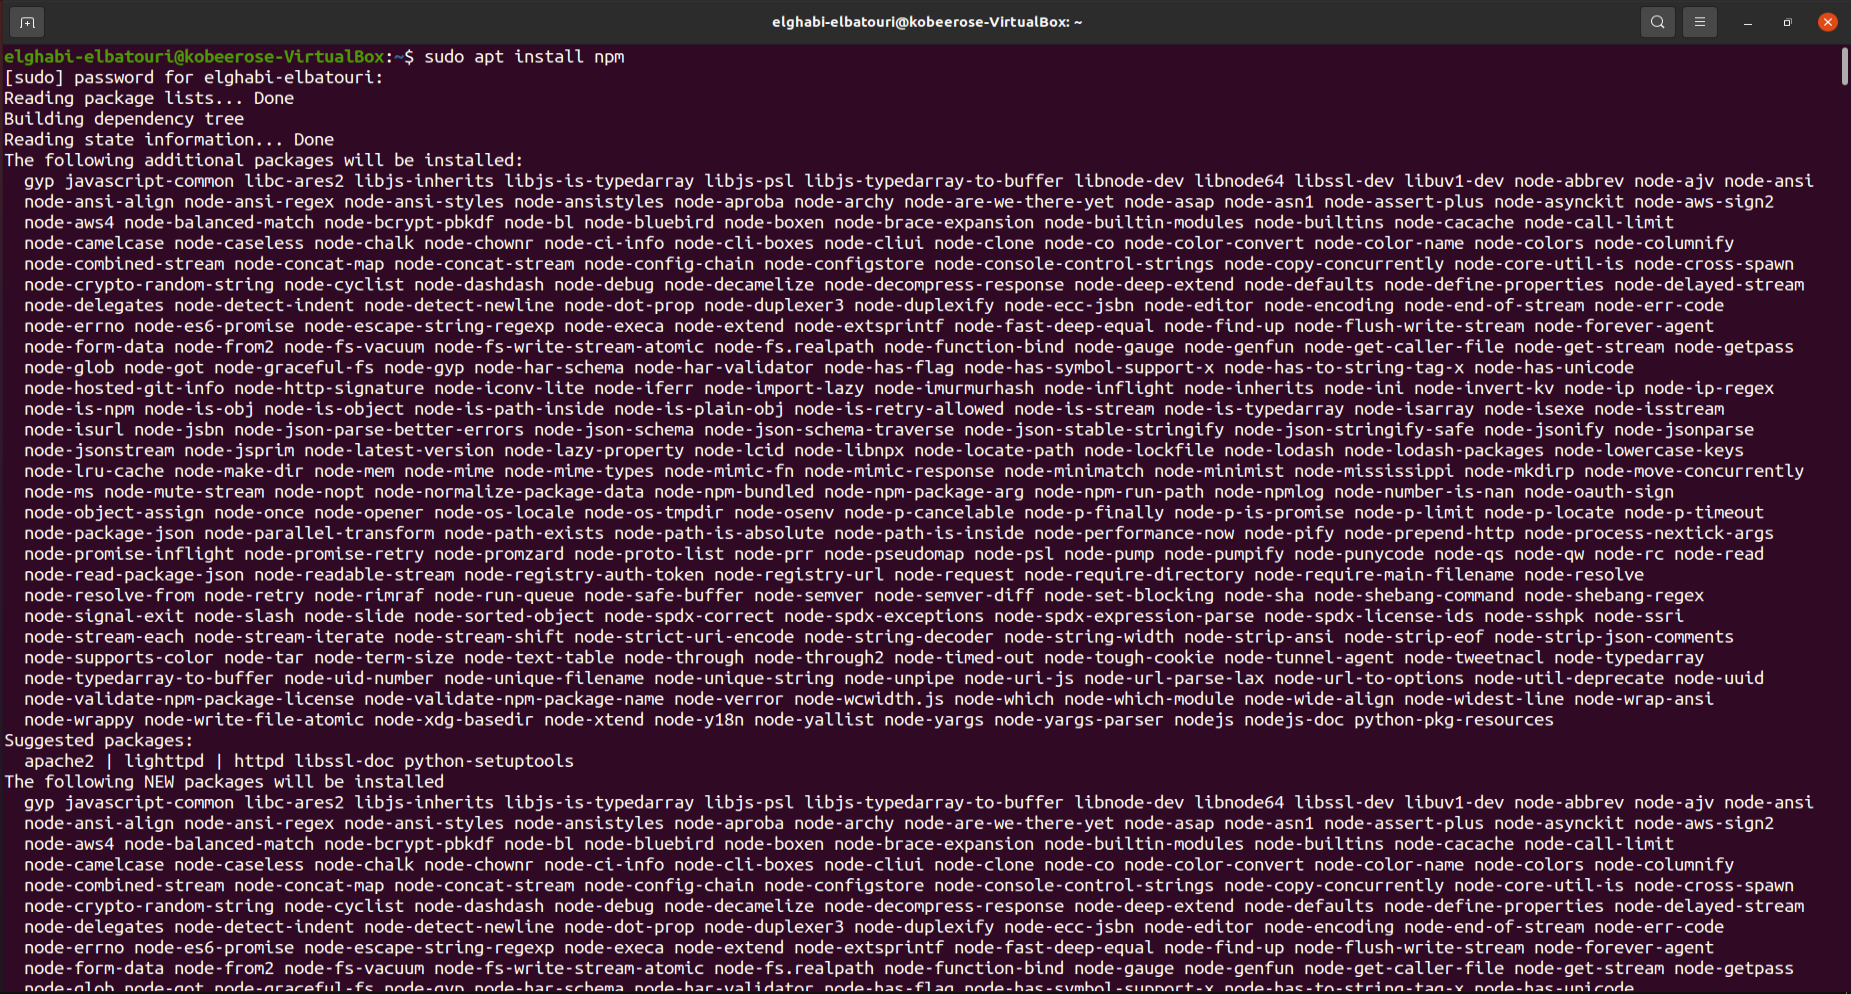
\includegraphics[width=1\linewidth]{Pictures/MongoDB/Node.js and MongoDB CRUD  application/Node.js installation/Install npm} 
\end{center} 
\caption{Install npm} 
\end{figure}  \FloatBarrier
\\

\par Lorem ipsum dolor sit amet, consectetur adipiscing elit. Aliquam facilisis massa quis orci volutpat, ut dictum tellus pulvinar. Nam vulputate diam a leo dignissim varius. Aenean nec tellus malesuada, tristique libero vitae, lacinia nibh. Donec quam libero, accumsan sollicitudin massa a, dictum gravida mauris
\\
\begin{figure}[!htb] 
\begin{center} 
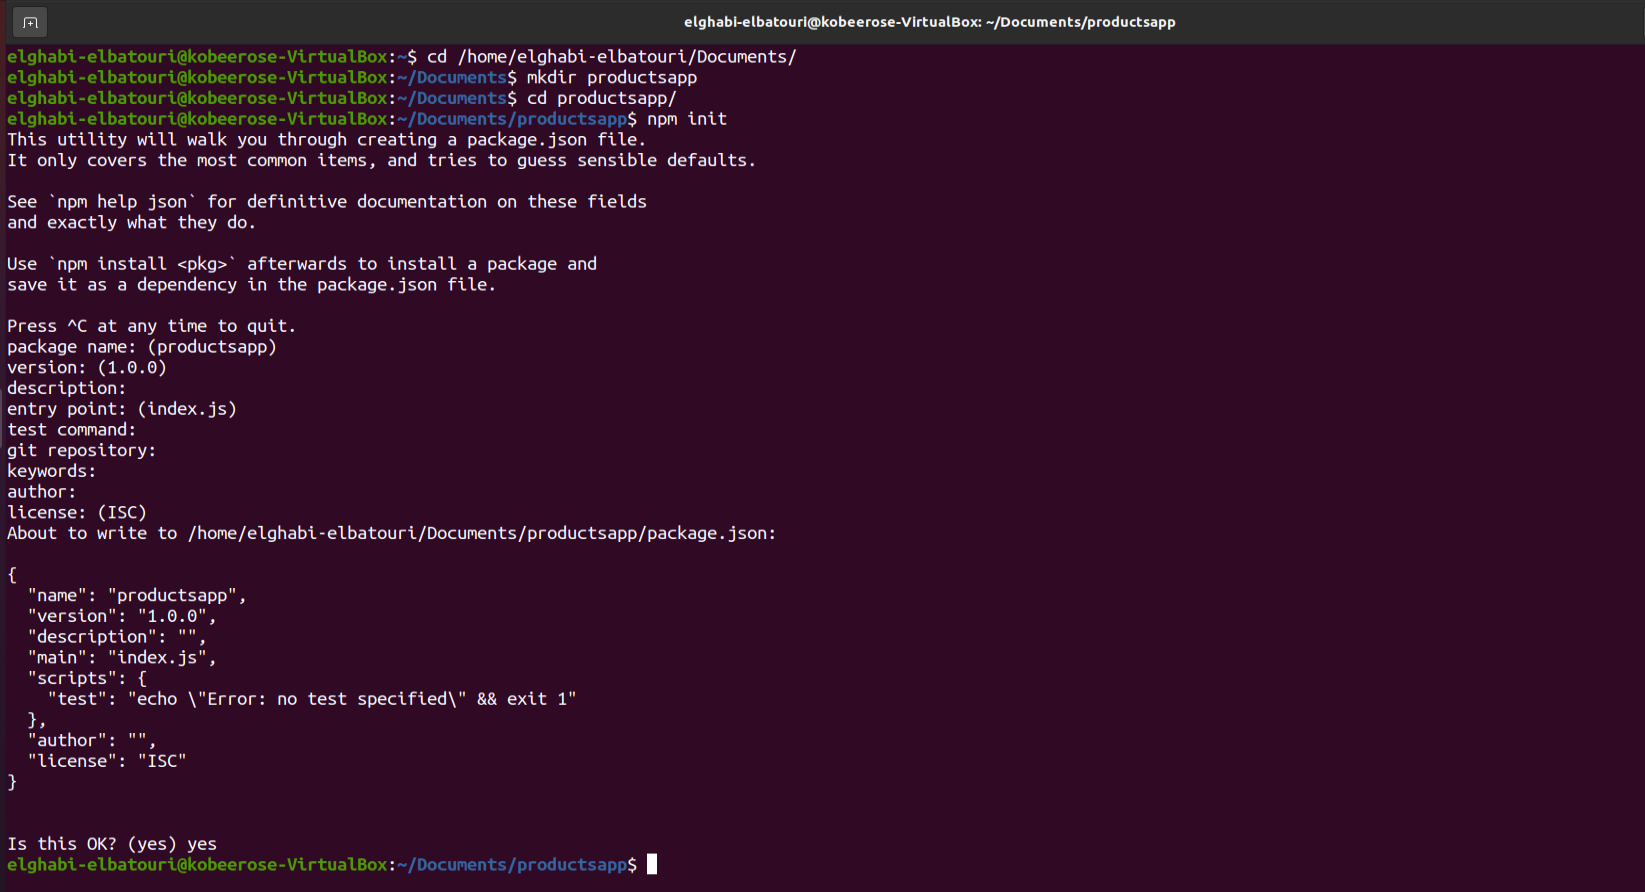
\includegraphics[width=1\linewidth]{Pictures/MongoDB/Node.js and MongoDB CRUD  application/Node.js installation/Creating package.json file} 
\end{center} 
\caption{Creating package.json file} 
\end{figure}  \FloatBarrier
\\

\par Lorem ipsum dolor sit amet, consectetur adipiscing elit. Aliquam facilisis massa quis orci volutpat, ut dictum tellus pulvinar. Nam vulputate diam a leo dignissim varius. Aenean nec tellus malesuada, tristique libero vitae, lacinia nibh. Donec quam libero, accumsan sollicitudin massa a, dictum gravida mauris
\\
\begin{figure}[!htb] 
\begin{center} 
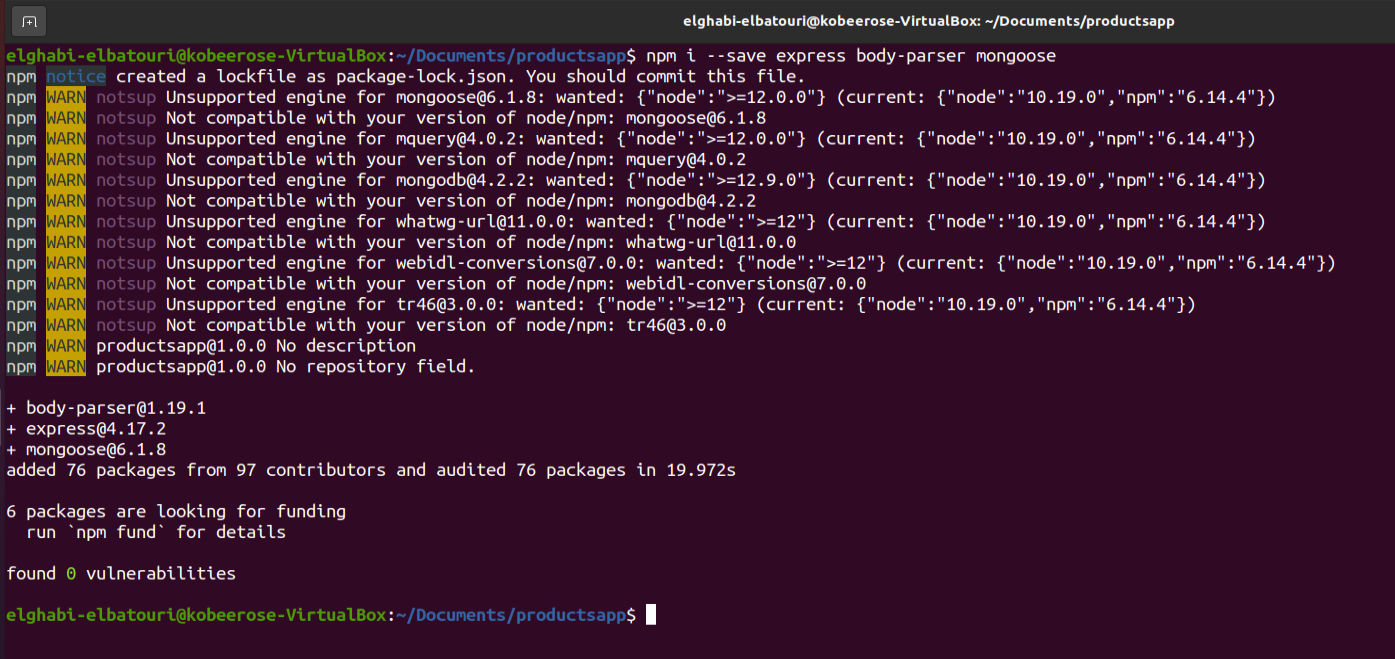
\includegraphics[width=1\linewidth]{Pictures/MongoDB/Node.js and MongoDB CRUD  application/Node.js installation/Installing dependencies} 
\end{center} 
\caption{Installing dependencies} 
\end{figure}  \FloatBarrier
\\

\par Lorem ipsum dolor sit amet, consectetur adipiscing elit. Aliquam facilisis massa quis orci volutpat, ut dictum tellus pulvinar. Nam vulputate diam a leo dignissim varius. Aenean nec tellus malesuada, tristique libero vitae, lacinia nibh. Donec quam libero, accumsan sollicitudin massa a, dictum gravida mauris
\\
\begin{figure}[!htb] 
\begin{center} 
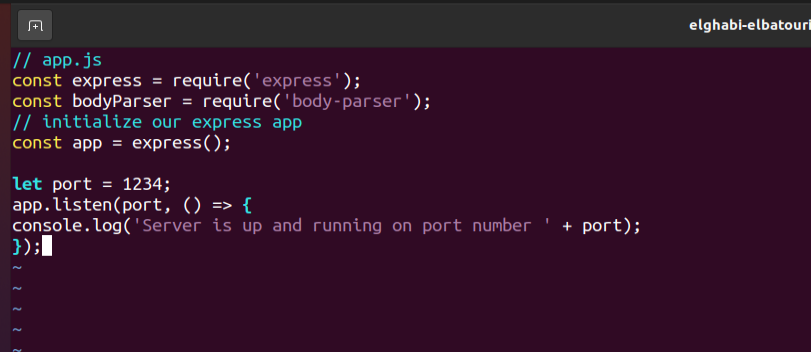
\includegraphics[width=1\linewidth]{Pictures/MongoDB/Node.js and MongoDB CRUD  application/Node.js installation/Creating app.js file} 
\end{center} 
\caption{Creating app.js file} 
\end{figure}  \FloatBarrier
\\

\par Lorem ipsum dolor sit amet, consectetur adipiscing elit. Aliquam facilisis massa quis orci volutpat, ut dictum tellus pulvinar. Nam vulputate diam a leo dignissim varius. Aenean nec tellus malesuada, tristique libero vitae, lacinia nibh. Donec quam libero, accumsan sollicitudin massa a, dictum gravida mauris
\\
\begin{figure}[!htb] 
\begin{center} 
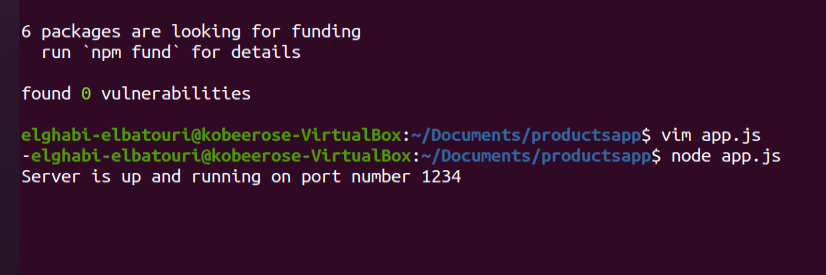
\includegraphics[width=1\linewidth]{Pictures/MongoDB/Node.js and MongoDB CRUD  application/Node.js installation/Running app.js} 
\end{center} 
\caption{Running app.js} 
\end{figure}  \FloatBarrier
\\
\section{Organization of the Node Application }
\par Lorem ipsum dolor sit amet, consectetur adipiscing elit. Aliquam facilisis massa quis orci volutpat, ut dictum tellus pulvinar. Nam vulputate diam a leo dignissim varius. Aenean nec tellus malesuada, tristique libero vitae, lacinia nibh. Donec quam libero, accumsan sollicitudin massa a, dictum gravida mauris
\\
\begin{figure}[!htb] 
\begin{center} 
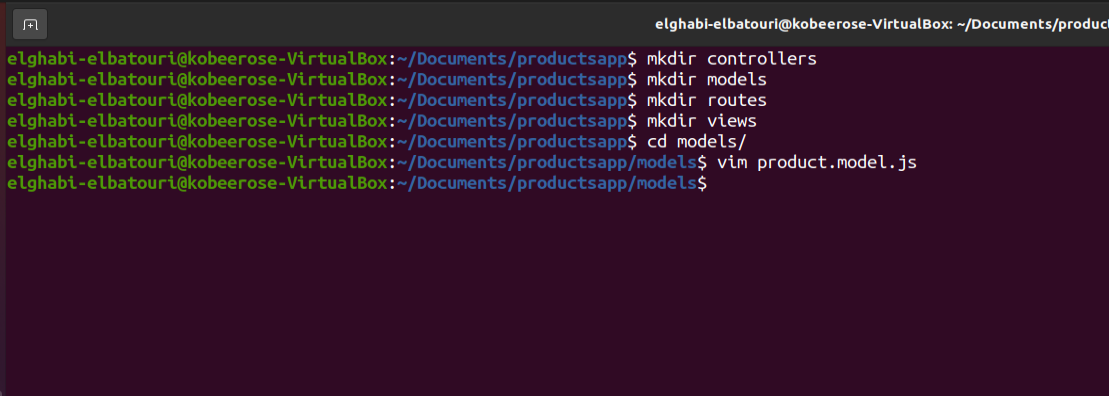
\includegraphics[width=1\linewidth]{Pictures/MongoDB/Node.js and MongoDB CRUD  application/Organization of the Node Application/Repositories for the app} 
\end{center} 
\caption{Repositories for the app} 
\end{figure}  \FloatBarrier
\\

\par Lorem ipsum dolor sit amet, consectetur adipiscing elit. Aliquam facilisis massa quis orci volutpat, ut dictum tellus pulvinar. Nam vulputate diam a leo dignissim varius. Aenean nec tellus malesuada, tristique libero vitae, lacinia nibh. Donec quam libero, accumsan sollicitudin massa a, dictum gravida mauris
\\
\begin{figure}[!htb] 
\begin{center} 
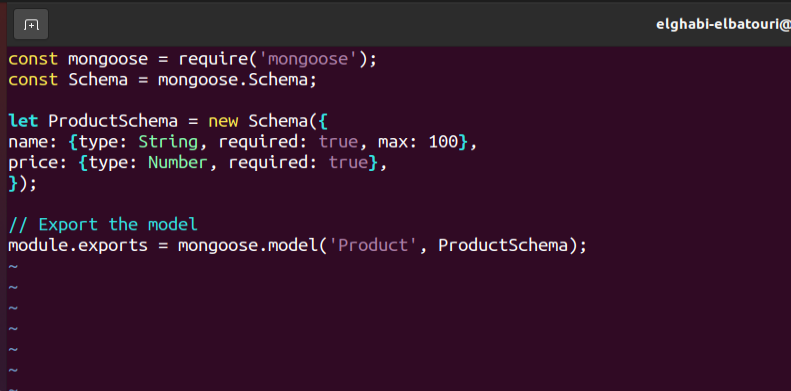
\includegraphics[width=1\linewidth]{Pictures/MongoDB/Node.js and MongoDB CRUD  application/Organization of the Node Application/Creating product.model.js file} 
\end{center} 
\caption{Creating product.model.js file} 
\end{figure}  \FloatBarrier
\\

\par Lorem ipsum dolor sit amet, consectetur adipiscing elit. Aliquam facilisis massa quis orci volutpat, ut dictum tellus pulvinar. Nam vulputate diam a leo dignissim varius. Aenean nec tellus malesuada, tristique libero vitae, lacinia nibh. Donec quam libero, accumsan sollicitudin massa a, dictum gravida mauris
\\
\begin{figure}[!htb] 
\begin{center} 
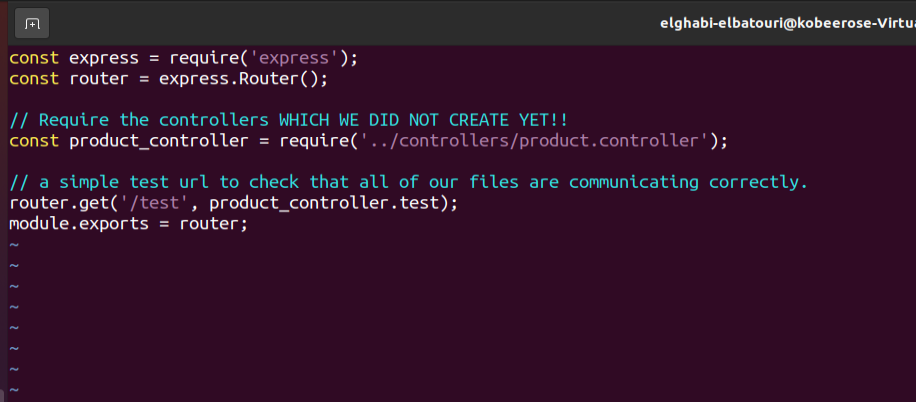
\includegraphics[width=1\linewidth]{Pictures/MongoDB/Node.js and MongoDB CRUD  application/Organization of the Node Application/Creating product.route.js file} 
\end{center} 
\caption{Creating product.route.js file} 
\end{figure}  \FloatBarrier
\\

\par Lorem ipsum dolor sit amet, consectetur adipiscing elit. Aliquam facilisis massa quis orci volutpat, ut dictum tellus pulvinar. Nam vulputate diam a leo dignissim varius. Aenean nec tellus malesuada, tristique libero vitae, lacinia nibh. Donec quam libero, accumsan sollicitudin massa a, dictum gravida mauris
\\
\begin{figure}[!htb] 
\begin{center} 
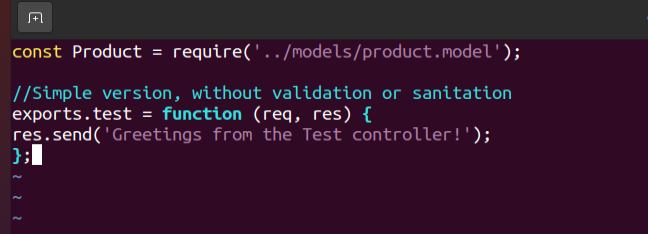
\includegraphics[width=1\linewidth]{Pictures/MongoDB/Node.js and MongoDB CRUD  application/Organization of the Node Application/Creating product.controller.js file} 
\end{center} 
\caption{Creating product.controller.js file} 
\end{figure}  \FloatBarrier
\\

\par Lorem ipsum dolor sit amet, consectetur adipiscing elit. Aliquam facilisis massa quis orci volutpat, ut dictum tellus pulvinar. Nam vulputate diam a leo dignissim varius. Aenean nec tellus malesuada, tristique libero vitae, lacinia nibh. Donec quam libero, accumsan sollicitudin massa a, dictum gravida mauris
\\
\begin{figure}[!htb] 
\begin{center} 
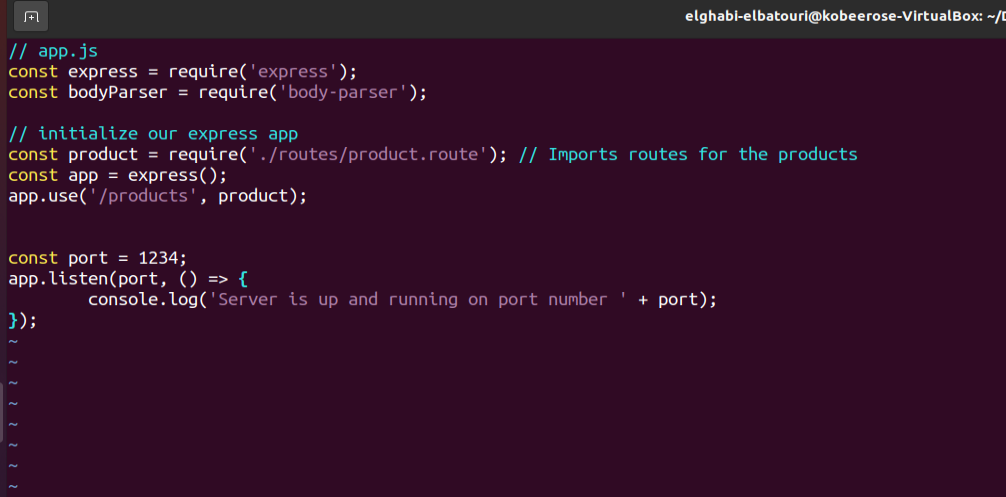
\includegraphics[width=1\linewidth]{Pictures/MongoDB/Node.js and MongoDB CRUD  application/Organization of the Node Application/Adding route to the app} 
\end{center} 
\caption{Adding route to the app} 
\end{figure}  \FloatBarrier
\\

\par Lorem ipsum dolor sit amet, consectetur adipiscing elit. Aliquam facilisis massa quis orci volutpat, ut dictum tellus pulvinar. Nam vulputate diam a leo dignissim varius. Aenean nec tellus malesuada, tristique libero vitae, lacinia nibh. Donec quam libero, accumsan sollicitudin massa a, dictum gravida mauris
\\
\begin{figure}[!htb] 
\begin{center} 
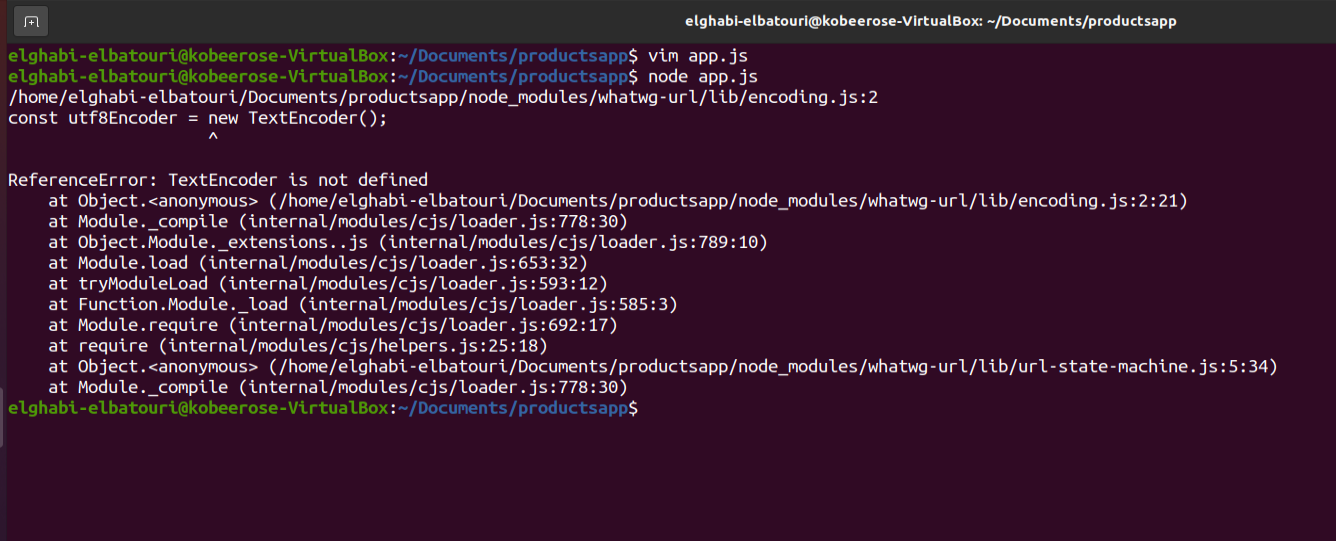
\includegraphics[width=1\linewidth]{Pictures/MongoDB/Node.js and MongoDB CRUD  application/Organization of the Node Application/Error when running the app} 
\end{center} 
\caption{Error when running the app} 
\end{figure}  \FloatBarrier
\\

\par Lorem ipsum dolor sit amet, consectetur adipiscing elit. Aliquam facilisis massa quis orci volutpat, ut dictum tellus pulvinar. Nam vulputate diam a leo dignissim varius. Aenean nec tellus malesuada, tristique libero vitae, lacinia nibh. Donec quam libero, accumsan sollicitudin massa a, dictum gravida mauris
\\
\begin{figure}[!htb] 
\begin{center} 
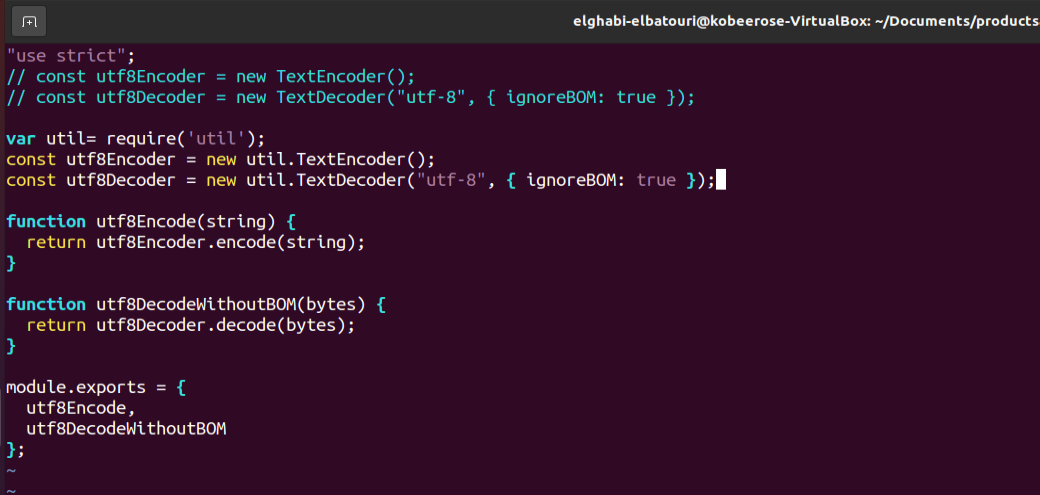
\includegraphics[width=1\linewidth]{Pictures/MongoDB/Node.js and MongoDB CRUD  application/Organization of the Node Application/Modifying encoding.js file} 
\end{center} 
\caption{Modifying encoding.js file} 
\end{figure}  \FloatBarrier
\\

\par Lorem ipsum dolor sit amet, consectetur adipiscing elit. Aliquam facilisis massa quis orci volutpat, ut dictum tellus pulvinar. Nam vulputate diam a leo dignissim varius. Aenean nec tellus malesuada, tristique libero vitae, lacinia nibh. Donec quam libero, accumsan sollicitudin massa a, dictum gravida mauris
\\
\begin{figure}[!htb] 
\begin{center} 
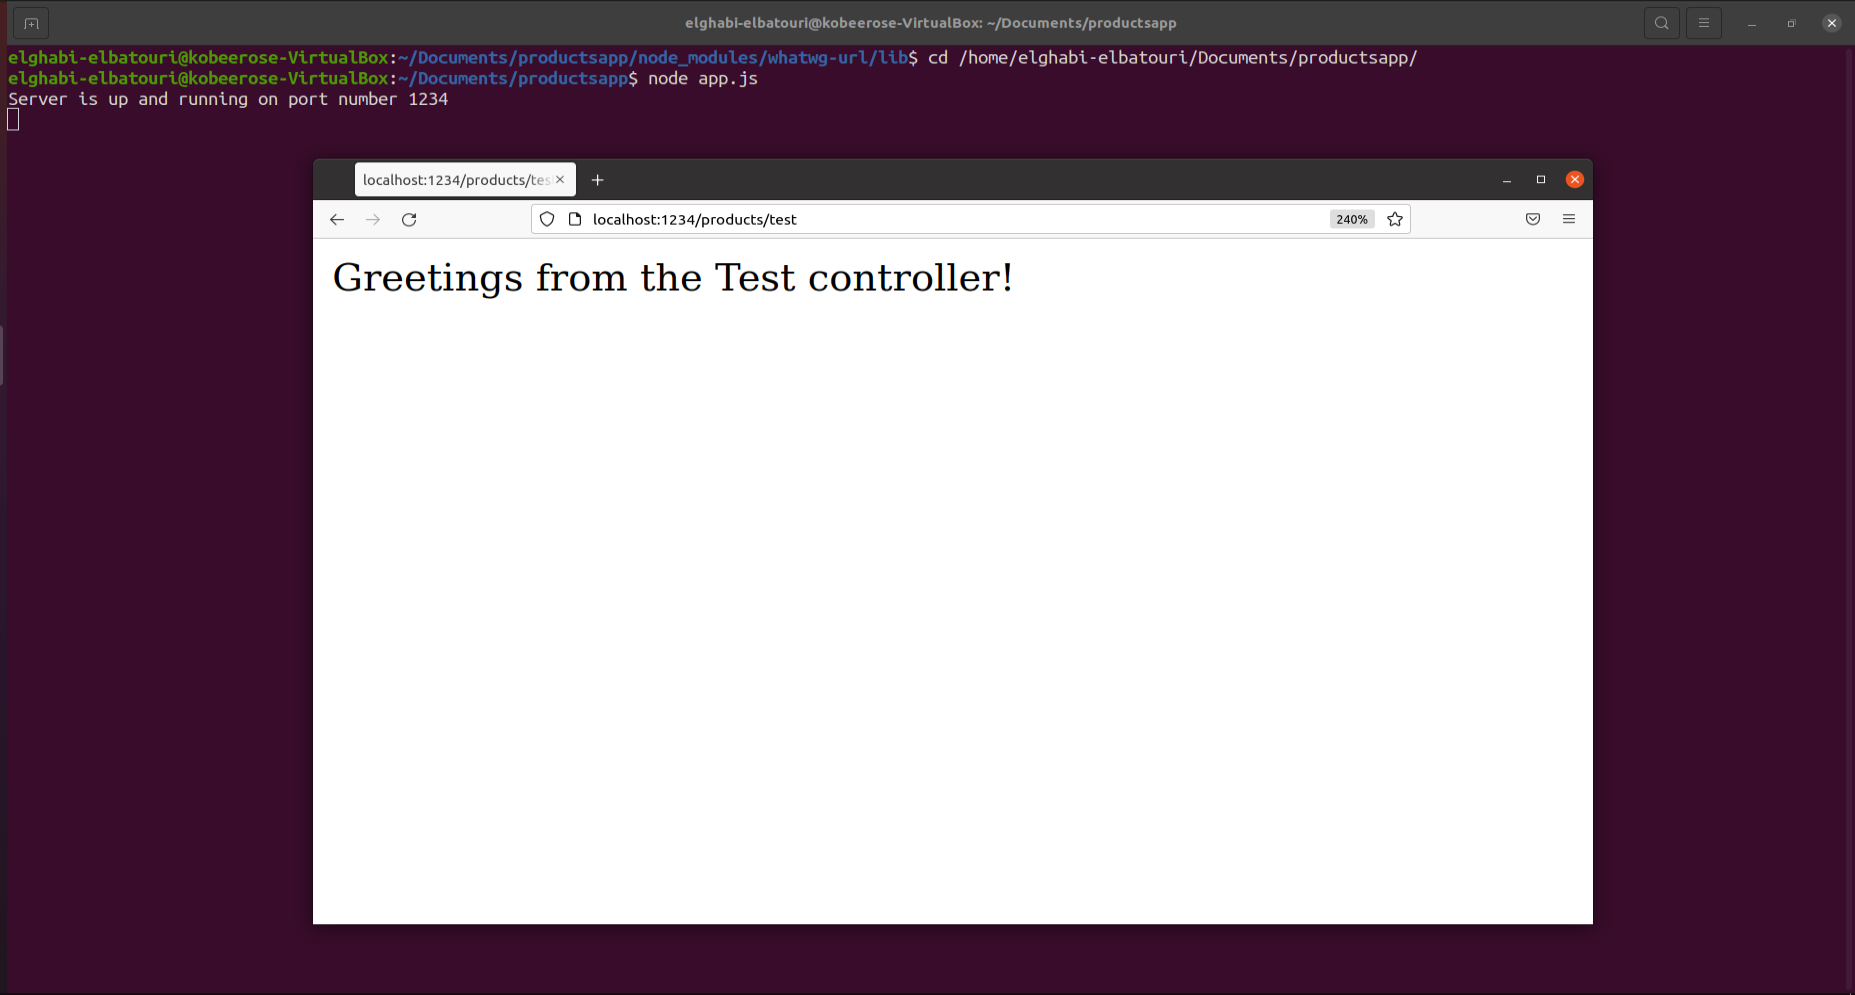
\includegraphics[width=1\linewidth]{Pictures/MongoDB/Node.js and MongoDB CRUD  application/Organization of the Node Application/Testing the app in browser} 
\end{center} 
\caption{Testing the app in browser} 
\end{figure}  \FloatBarrier
\\
\section{Postman }
\par Lorem ipsum dolor sit amet, consectetur adipiscing elit. Aliquam facilisis massa quis orci volutpat, ut dictum tellus pulvinar. Nam vulputate diam a leo dignissim varius. Aenean nec tellus malesuada, tristique libero vitae, lacinia nibh. Donec quam libero, accumsan sollicitudin massa a, dictum gravida mauris
\\
\begin{figure}[!htb] 
\begin{center} 
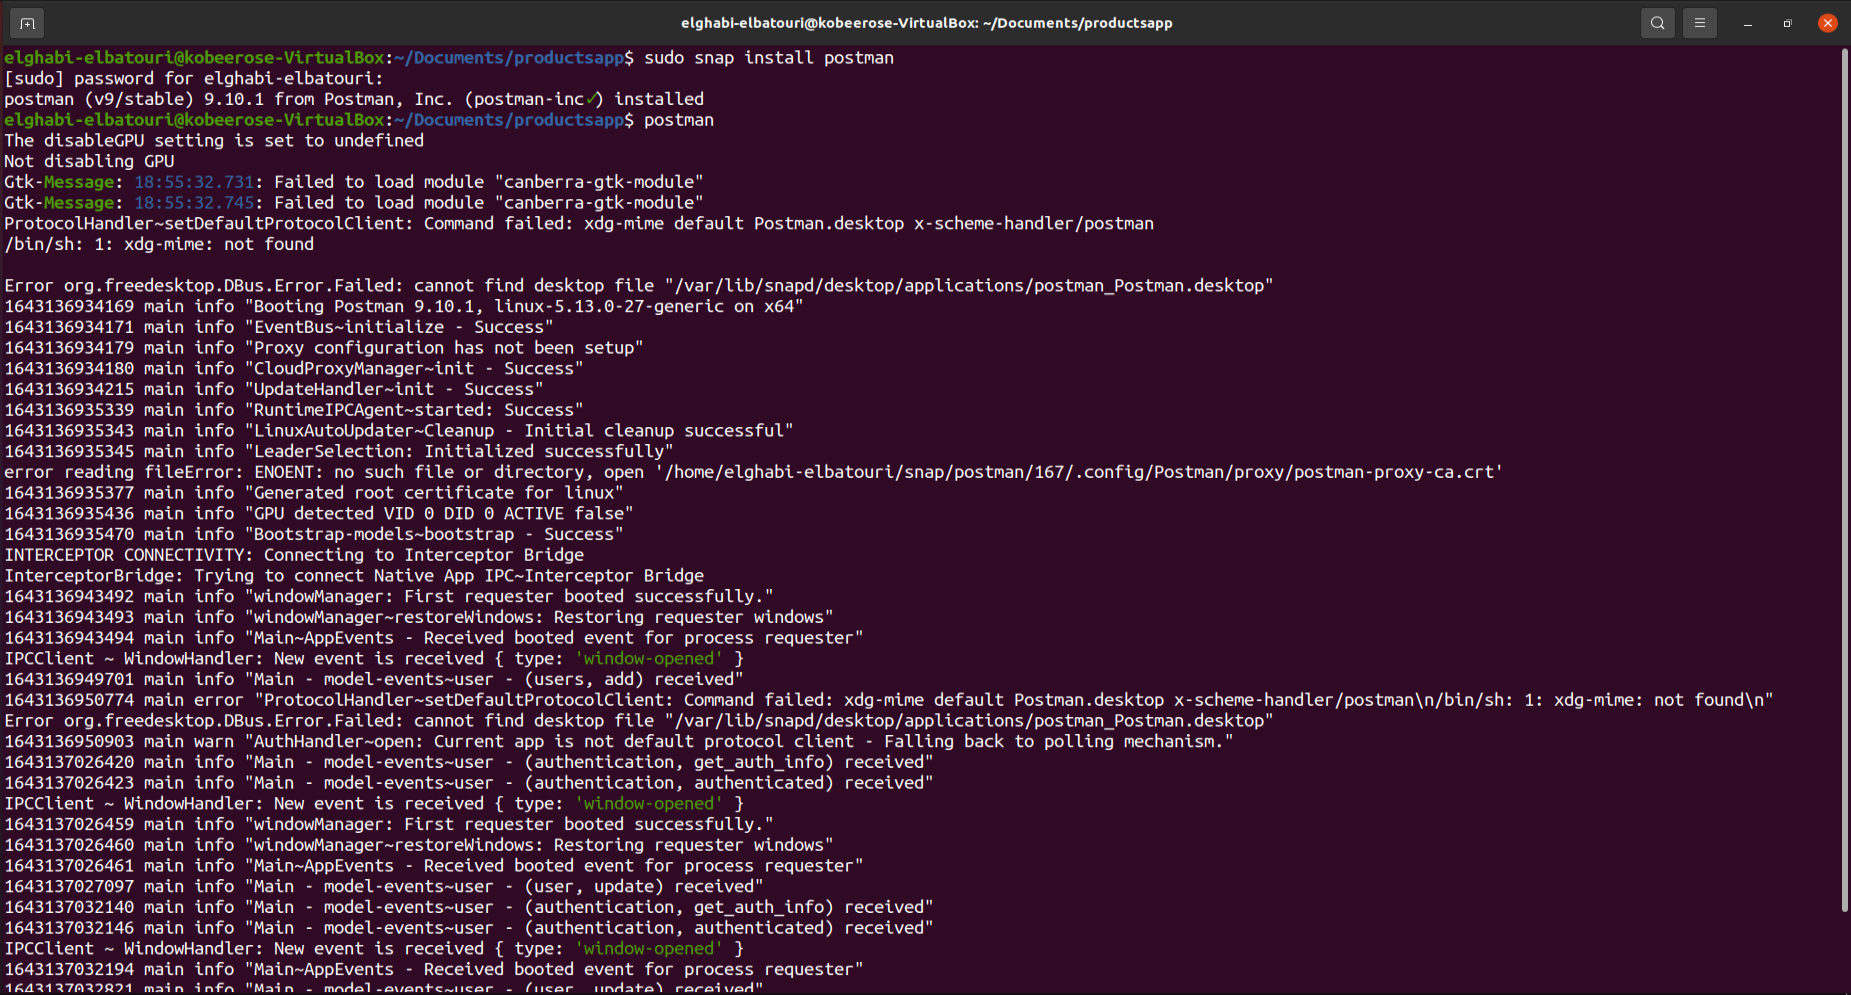
\includegraphics[width=1\linewidth]{Pictures/MongoDB/Node.js and MongoDB CRUD  application/Postman/Installing and running Postman} 
\end{center} 
\caption{Installing and running Postman} 
\end{figure}  \FloatBarrier
\\

\par Lorem ipsum dolor sit amet, consectetur adipiscing elit. Aliquam facilisis massa quis orci volutpat, ut dictum tellus pulvinar. Nam vulputate diam a leo dignissim varius. Aenean nec tellus malesuada, tristique libero vitae, lacinia nibh. Donec quam libero, accumsan sollicitudin massa a, dictum gravida mauris
\\
\begin{figure}[!htb] 
\begin{center} 
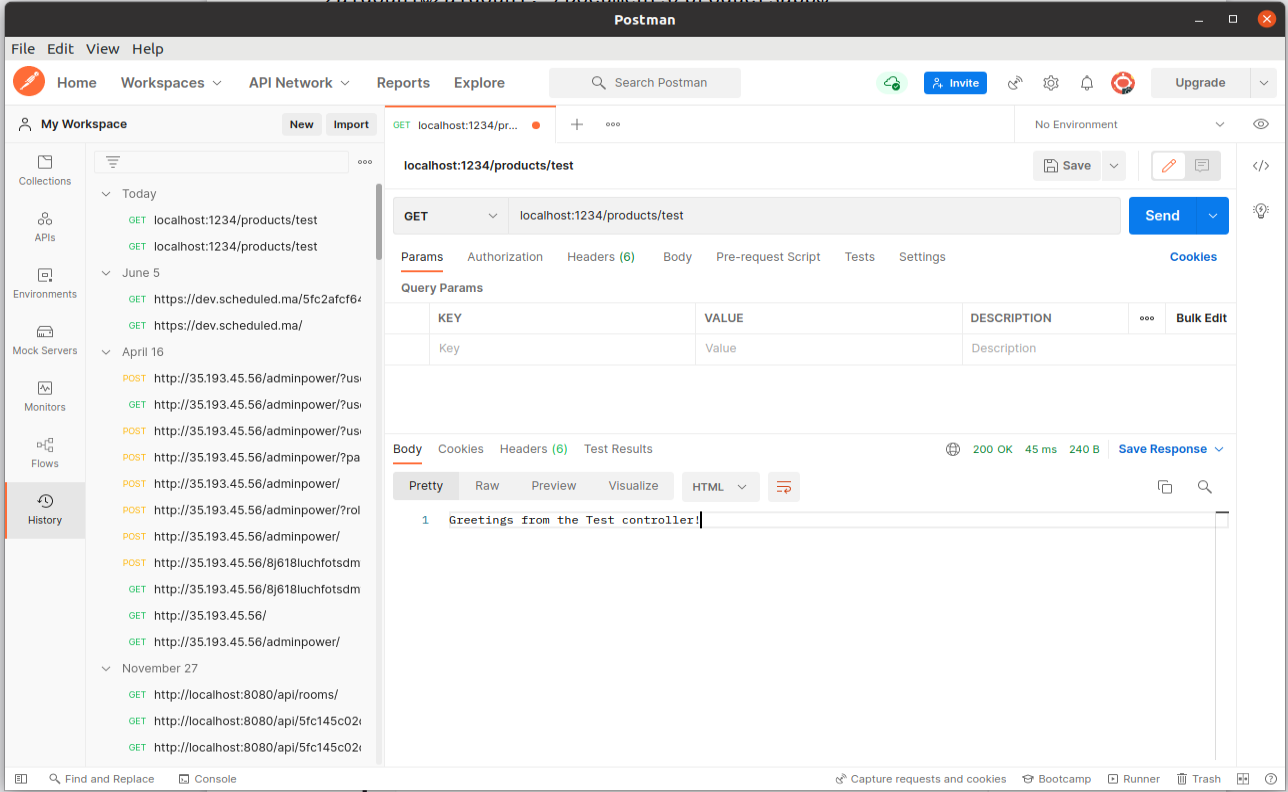
\includegraphics[width=1\linewidth]{Pictures/MongoDB/Node.js and MongoDB CRUD  application/Postman/Testing GET request with Postman} 
\end{center} 
\caption{Testing GET request with Postman} 
\end{figure}  \FloatBarrier
\\

\par Lorem ipsum dolor sit amet, consectetur adipiscing elit. Aliquam facilisis massa quis orci volutpat, ut dictum tellus pulvinar. Nam vulputate diam a leo dignissim varius. Aenean nec tellus malesuada, tristique libero vitae, lacinia nibh. Donec quam libero, accumsan sollicitudin massa a, dictum gravida mauris
\\
\begin{figure}[!htb] 
\begin{center} 
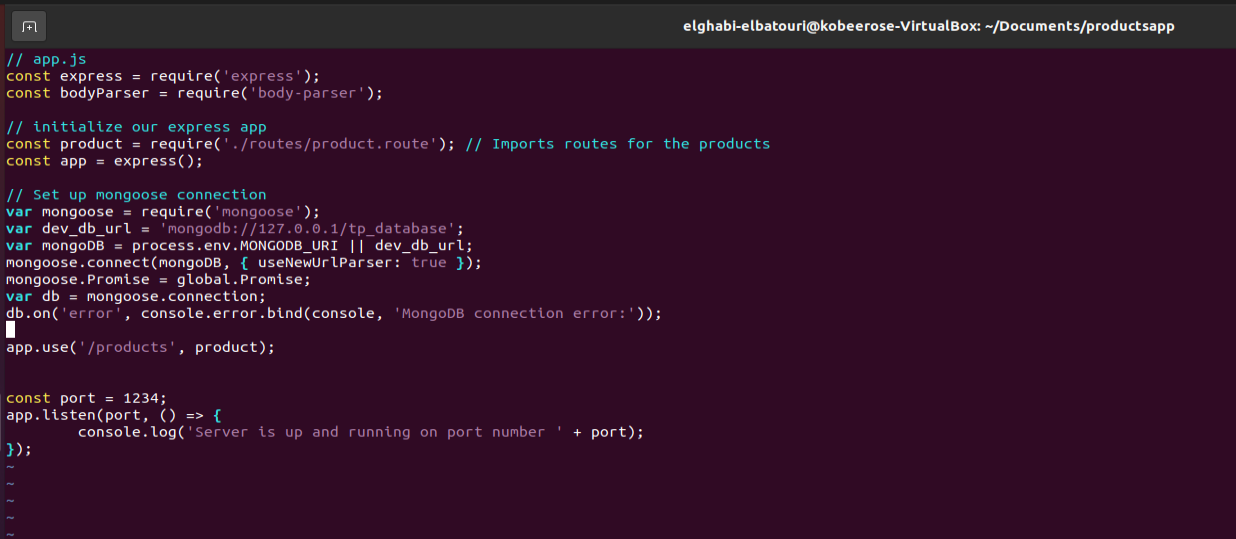
\includegraphics[width=1\linewidth]{Pictures/MongoDB/Node.js and MongoDB CRUD  application/Postman/Connection to mongoose} 
\end{center} 
\caption{Connection to mongoose} 
\end{figure}  \FloatBarrier
\\

\par Lorem ipsum dolor sit amet, consectetur adipiscing elit. Aliquam facilisis massa quis orci volutpat, ut dictum tellus pulvinar. Nam vulputate diam a leo dignissim varius. Aenean nec tellus malesuada, tristique libero vitae, lacinia nibh. Donec quam libero, accumsan sollicitudin massa a, dictum gravida mauris
\\
\begin{figure}[!htb] 
\begin{center} 
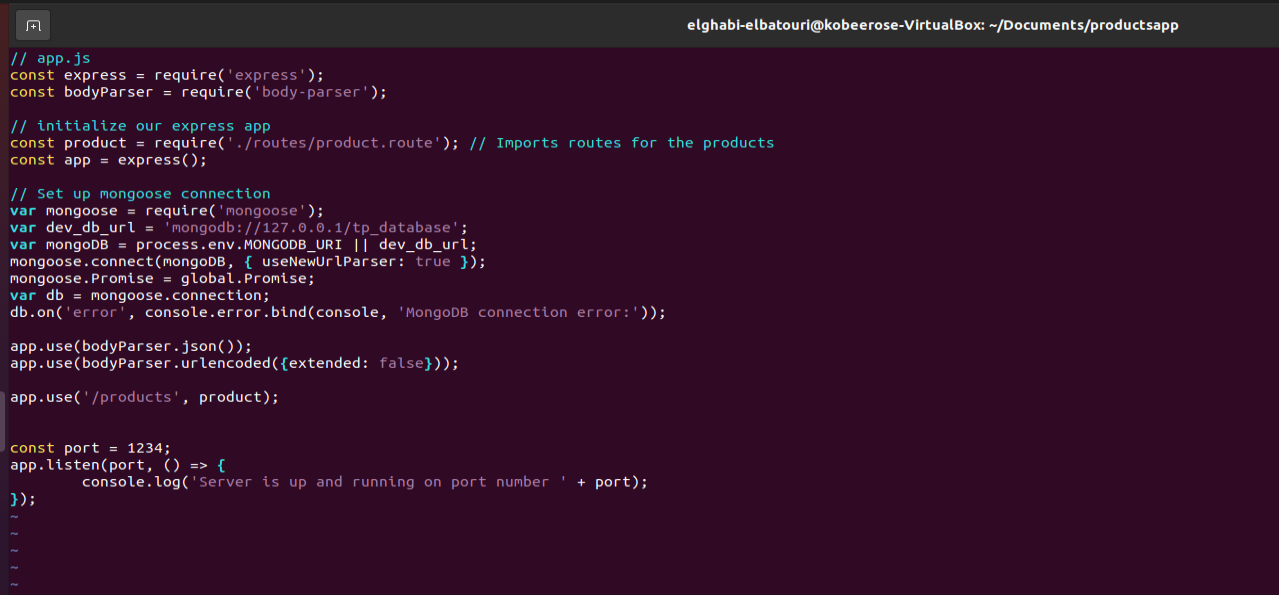
\includegraphics[width=1\linewidth]{Pictures/MongoDB/Node.js and MongoDB CRUD  application/Postman/Body Parser package} 
\end{center} 
\caption{Body Parser package} 
\end{figure}  \FloatBarrier
\\

\end{spacing}